
\section{\LaTeX\ }


This section walks you through the most critical, time-consuming, less-rewarding steps of  the download \& installation of the LaTeX distribution, to the point where you can compile and edit your own documents. 
\paragraph{}
There are two things that you need in order to do so:
\begin{itemize}
\item[1.] The \LaTeX\ distribution: the (huge) software package that will compile your raw .tex document and turn them into  neat pdf documents.
\item[2.]  The TeX editor. This is the software that you will use to create and edit .tex documents. It also provides an interface with the compiler.
\end{itemize}
\paragraph{}
The procedure is slightly different depending on whether you are using Windows or MacOS.

\subsection{Retrieving the \LaTeX\ Distribution }

\subsubsection*{Windows}
Two versions of the \LaTeX\ distribution installer are available on the  \href{http://www.miktex.org/download
}{\textcolor{blue}{MikTeX website}}



\begin{itemize}
\item If your computer is less than two years old,
you can download the MiKTeX 2.9.5870 Net Installer 64-bits executable
\item If you are not sure whether you can run the 64-bits executable, 
download the MiKTeX 2.9.5870 Net 32-bits executable 
\end{itemize}


\begin{itemize}
\item[1.] Run the installer once the file is downloaded.
\item[2.] When asked, click ‘Download MiKTeX’ to download the distribution.
\item[3.] When asked whether the executable should download the Basic or Complete MiKTeX distribution, choose Complete
\item[4.] Choose the folder where the installation files will be downloaded
\item[5.] Pick a download source geographically close from CU in the server list that should pop up
\item[6.] Start the download...
\end{itemize}
...which might take a while...
\begin{itemize}
\item[7.] Once the download is over, go to the folder where you saved the \LaTeX\ distribution files. Look for setup-2.9.3959.exe (the only executable file in this folder) and run it.
\item[8.] Once the installation process is over, you have a complete \LaTeX\ distribution installed on your PC and are almost good to go!
\end{itemize}

\subsubsection{MacOS}
\href{https://tug.org/mactex/mactex-download.html}{\textcolor{blue}{The MacTex distribution}} can be found there. Click on the link at the center of the page to get the whole distribution. The file weighs 2.5 GB so the download might take a while .

\subsection{Getting the Tex Editor}
From my own experience, I strongly recommend
\href{http://www.xm1math.net/texmaker/}{\textcolor{blue}{Texmaker}}. The interface is neat and the autocomplete functionality (that predicts the rest of the command you are typing) rocks.\\
This software works on Windows, MacOS and Linux. The version you need can be found on the download page. Installing Texmaker does not require any special instructions so you should be fine!

\subsection{Editing and compiling this tutorial}

First of all, download the following \href{https://drive.google.com/file/d/0Bzf79yzZcPJJNVhKNFBxWGs1aEE/view?usp=sharing}{archive} and extract it into a folder of your choice.

The \textit{preamble.tex} file lists all the packages that are needed in order to compile some commands that would otherwise be unknown to the Latex compiler. I have been using Latex and constantly updating this list of packages for nearly 4 years, so it should be comprehensive enough now\footnote{The \textit{float} package that you will see listed in the preamble is one of these packages that come in handy. Without it, including figures in your document can lead to layout disasters... }.

Once this is done, open Texmaker. Figure \ref{fig:texmaker_menu} shows what you should see as you have no tex document currently opened.

\begin{figure}[H]
\centering
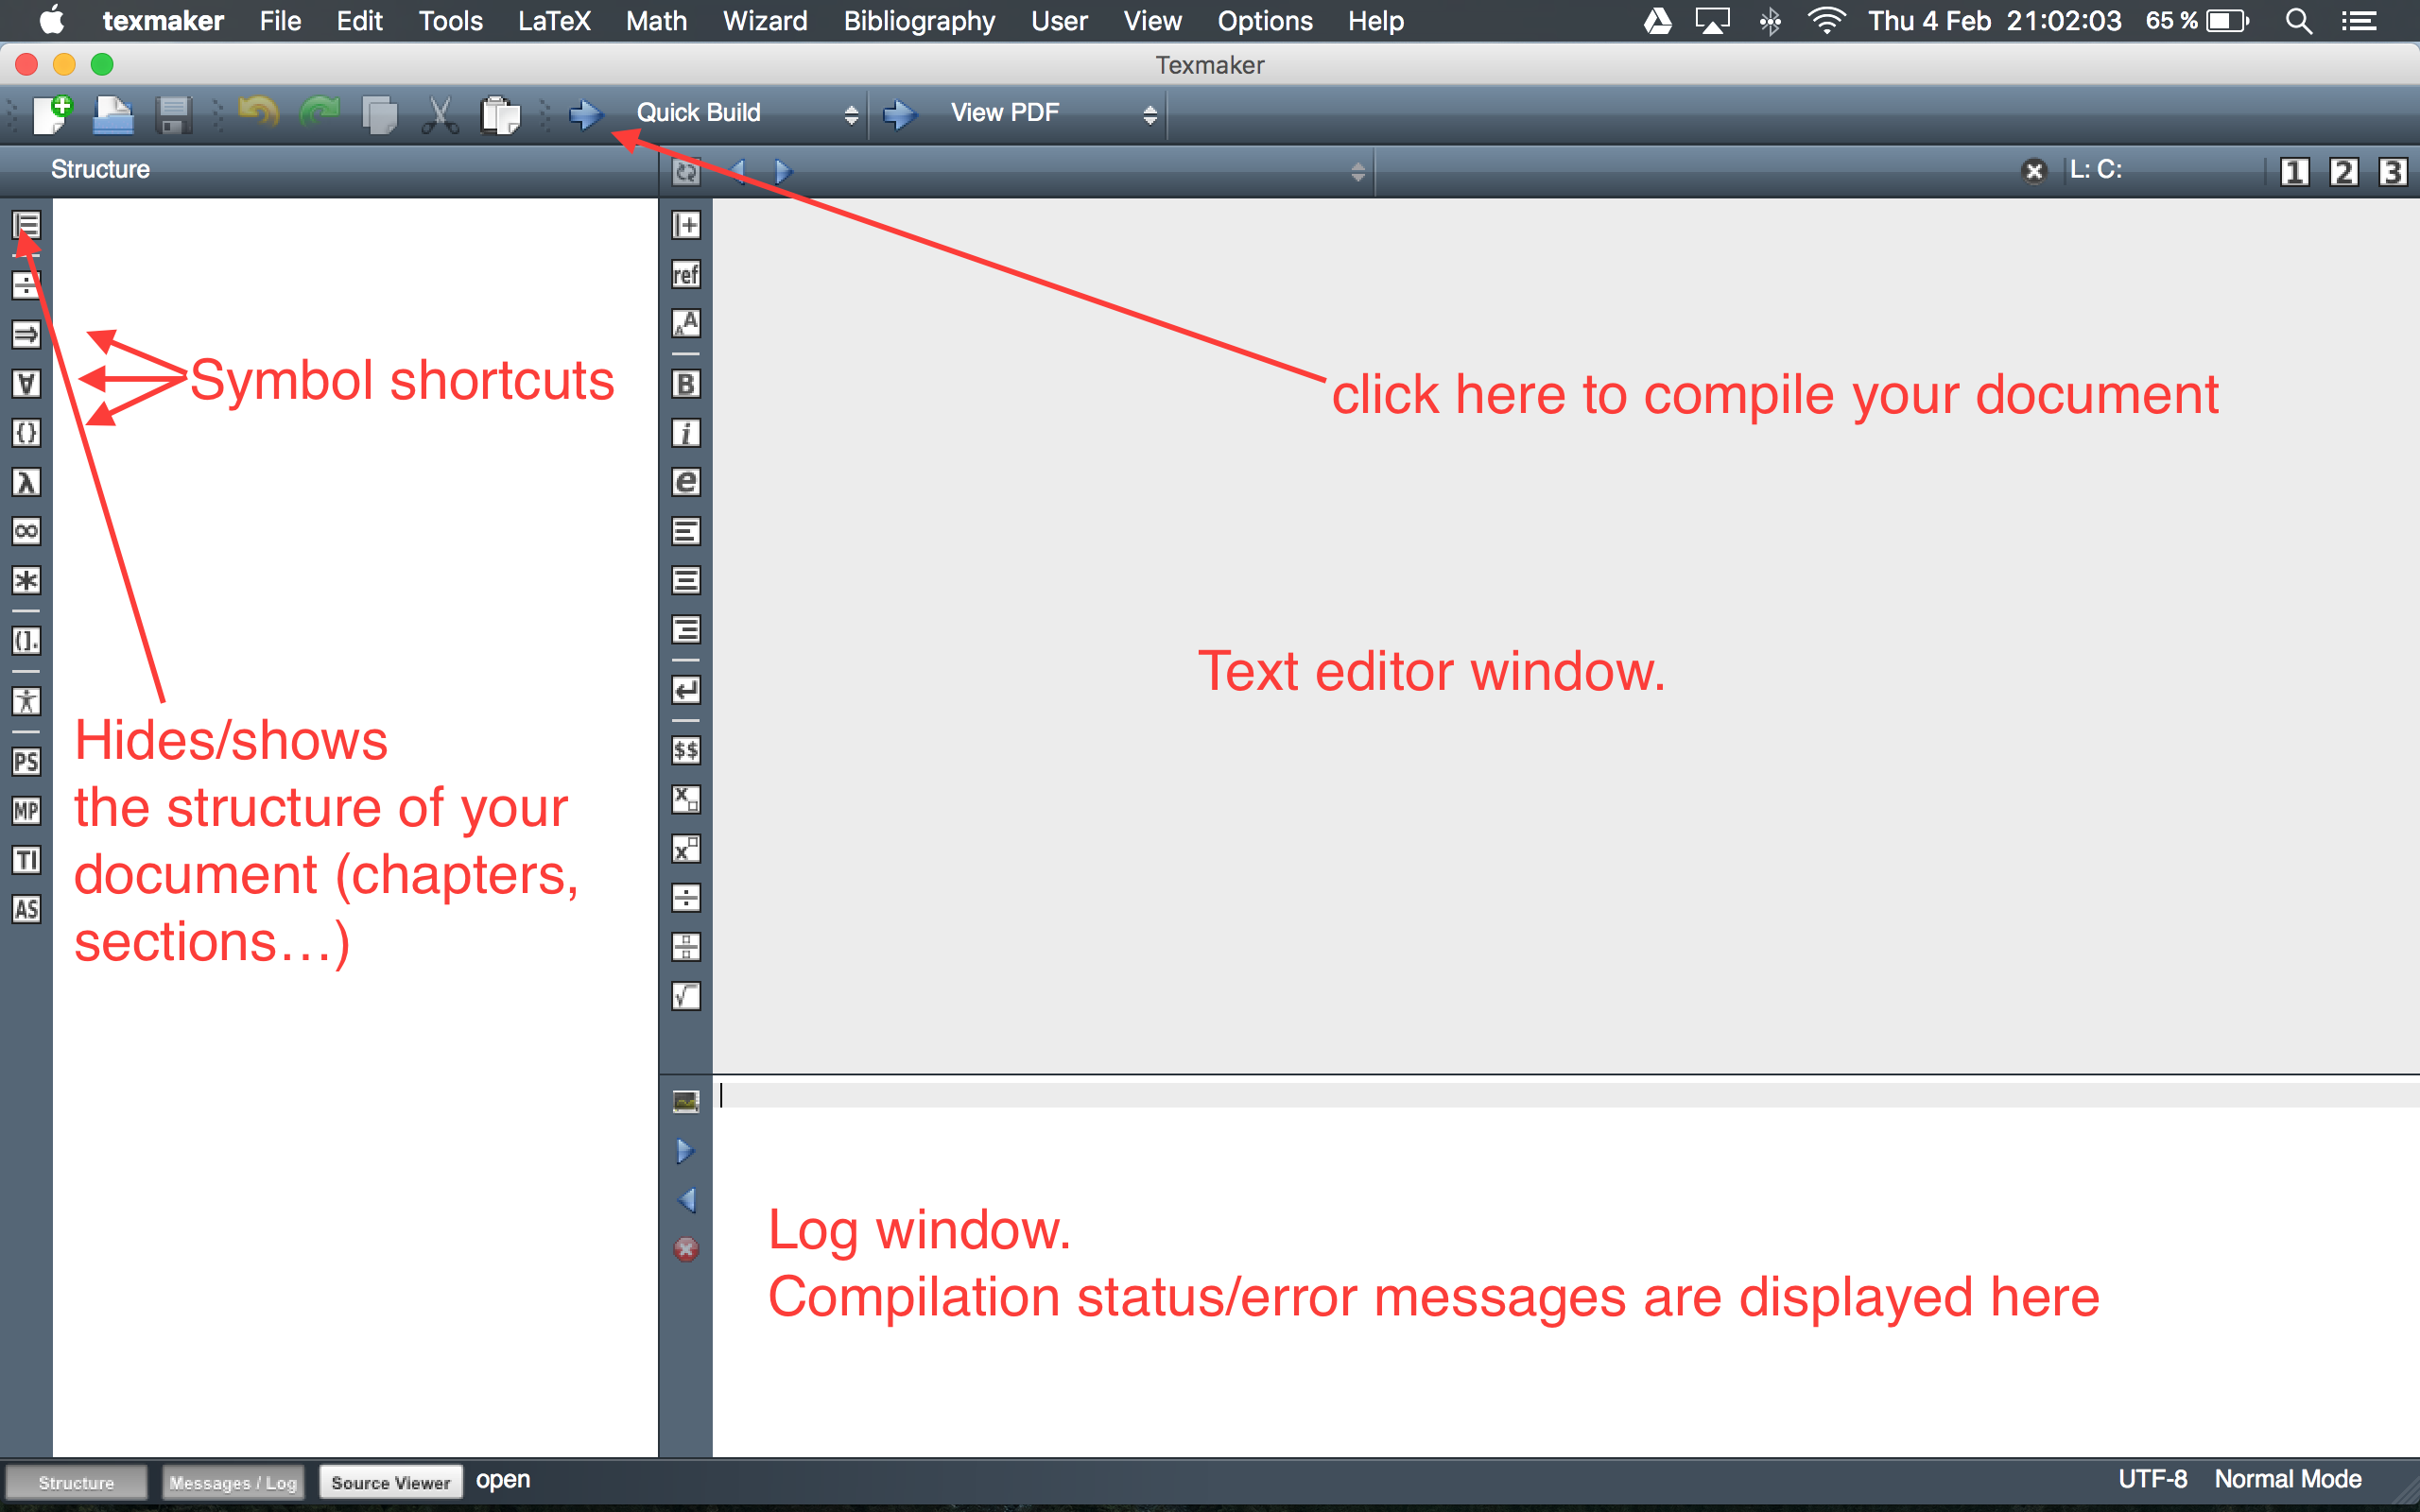
\includegraphics[scale=0.38]{texmaker_menu}
\caption{Main menu}
\label{fig:texmaker_menu}
\end{figure}

Opening the tutorial.tex file should get you the same view as on Figure \ref{fig:opened_document}:

\begin{figure}[H]
\centering
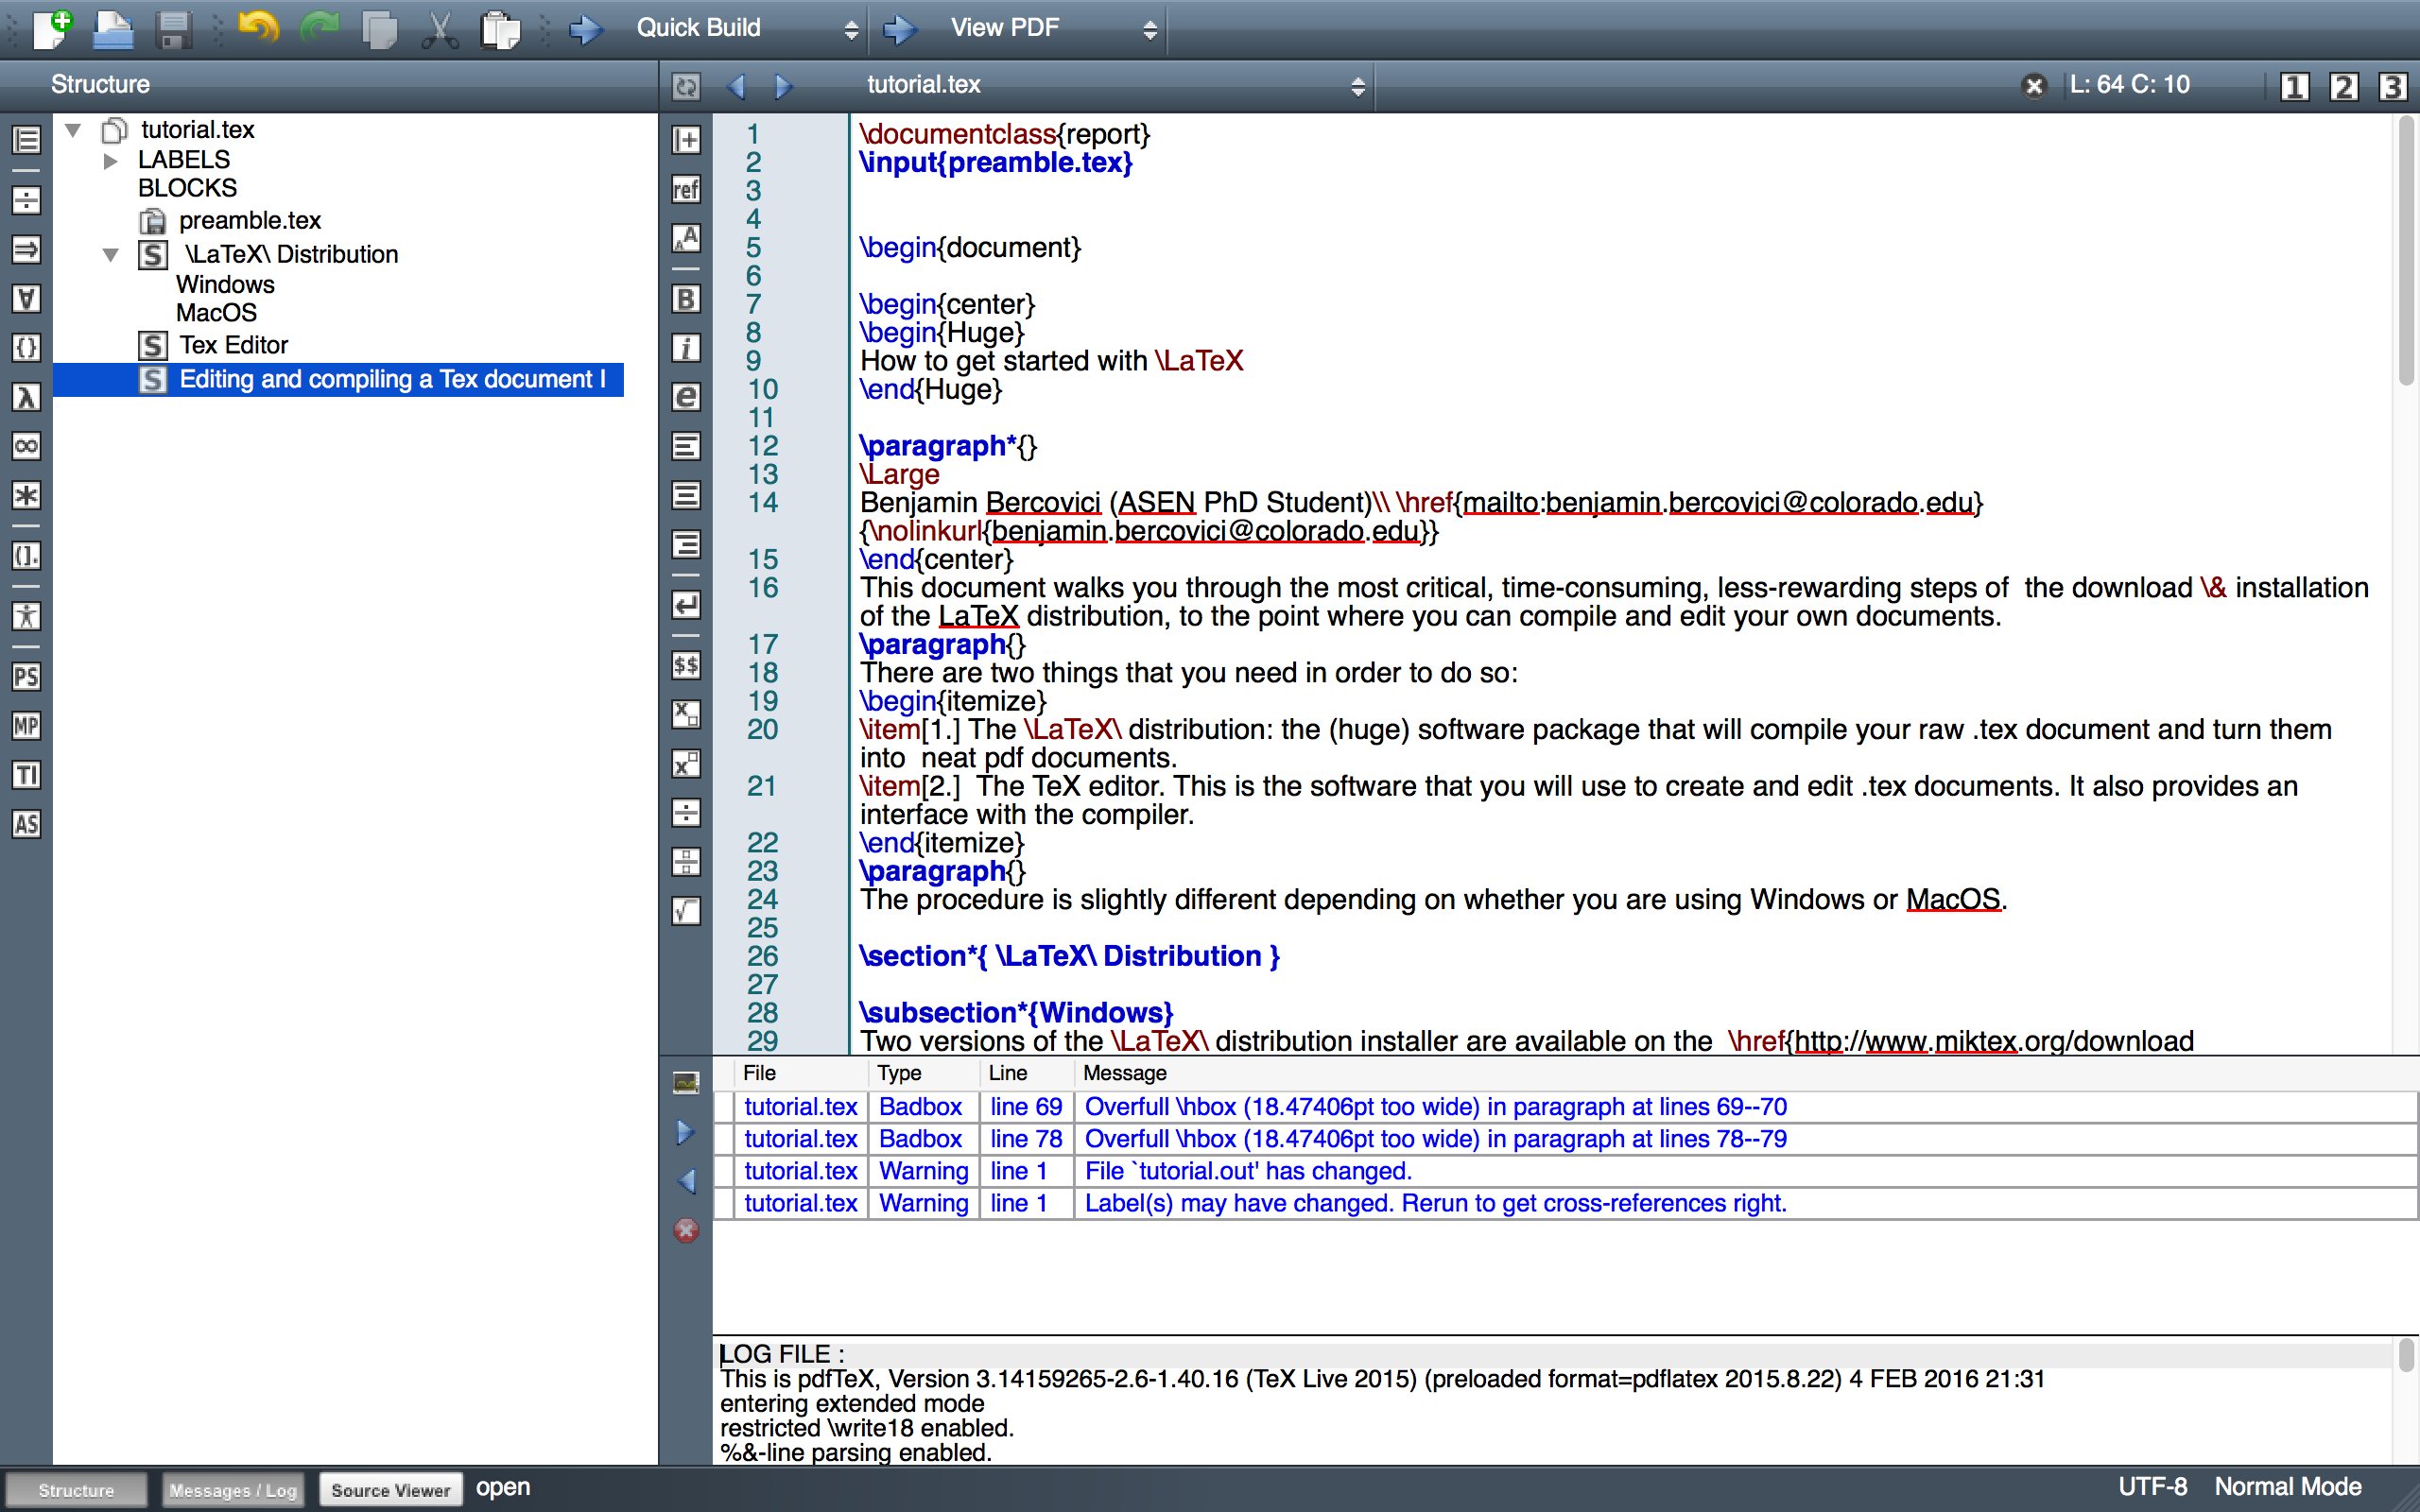
\includegraphics[scale=0.38]{opened_document}
\caption{Texmaker displaying the \textit{tutorial.tex} file. Note that the document structure automatically appears on the left side of the window}
\label{fig:opened_document}
\end{figure}
If you take a look at the very top of the document, you will recognize the \textit{preamble.tex} file that I mentioned before. The \textit{$\setminus$input\{preamble.tex\}} command will - as the name suggests - have \textit{tutorial.tex} including the content of \textit{preamble.tex}. It is equivalent to copying the content of \textit{preamble.tex} and pasting it into \textit{tutorial.tex}. Because the latter would be rather messy, listing all the packages you will use in an external file and using the input command is a much better practice.\\

Note that everything that begins with a $\setminus$\footnote{The key that corresponds to this symbol is the one right above the Enter/Return Key.} is a \LaTeX\ command. This $\setminus$ tells the compiler that whatever follows this symbol has to be interpreted. Plain text is just considered as is. \\
Clicking on the \textit{Quick Build} button will run the compiler, that will process the .tex file and generate a \textit{tutorial.pdf} document in the same folder as the \textit{tutorial.tex} file

\subsection{Maths and \LaTeX }
There are thousands of tutorials available on the web addressing this topic. The greatest understatement of the day would be to say that \LaTeX\ is really well suited to maths typesetting. Several examples based off former homeworks of mine are available \href{https://drive.google.com/file/d/0Bzf79yzZcPJJSnJKOFdrLVhtSG8/view?usp=sharing}{there}.

I strongly encourage you to open the document, compile it, see the pdf output, and then take a closer look at the .tex file to understand how mathematical expressions are formatted.
\subsection*{Resources}
Dr. Schaub has listed a number of references on \href{http://hanspeterschaub.info/AVS-LaTeX.html}{his website} which I encourage you to use. There is in particular a Latex cheat sheet that could come in handy.  
